% Created by tikzDevice version 0.12.3.1 on 2021-12-06 10:54:56
% !TEX encoding = UTF-8 Unicode
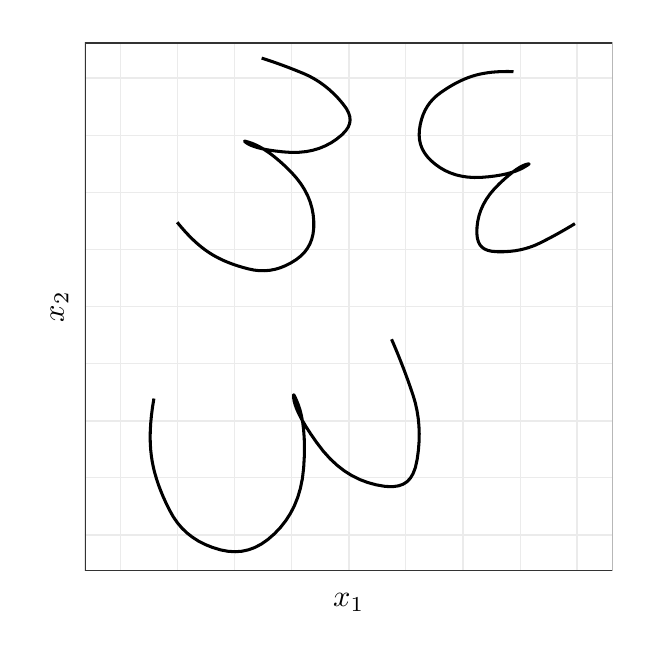
\begin{tikzpicture}[x=1pt,y=1pt]
\definecolor{fillColor}{RGB}{255,255,255}
\path[use as bounding box,fill=fillColor,fill opacity=0.00] (0,0) rectangle (216.81,216.81);
\begin{scope}
\path[clip] (  0.00,  0.00) rectangle (216.81,216.81);
\definecolor{drawColor}{RGB}{255,255,255}
\definecolor{fillColor}{RGB}{255,255,255}

\path[draw=drawColor,line width= 0.6pt,line join=round,line cap=round,fill=fillColor] (  0.00,  0.00) rectangle (216.81,216.81);
\end{scope}
\begin{scope}
\path[clip] ( 20.71, 20.71) rectangle (211.31,211.31);
\definecolor{fillColor}{RGB}{255,255,255}

\path[fill=fillColor] ( 20.71, 20.71) rectangle (211.31,211.31);
\definecolor{drawColor}{gray}{0.92}

\path[draw=drawColor,line width= 0.3pt,line join=round] ( 20.71, 54.13) --
	(211.31, 54.13);

\path[draw=drawColor,line width= 0.3pt,line join=round] ( 20.71, 95.38) --
	(211.31, 95.38);

\path[draw=drawColor,line width= 0.3pt,line join=round] ( 20.71,136.64) --
	(211.31,136.64);

\path[draw=drawColor,line width= 0.3pt,line join=round] ( 20.71,177.89) --
	(211.31,177.89);

\path[draw=drawColor,line width= 0.3pt,line join=round] ( 54.13, 20.71) --
	( 54.13,211.31);

\path[draw=drawColor,line width= 0.3pt,line join=round] ( 95.38, 20.71) --
	( 95.38,211.31);

\path[draw=drawColor,line width= 0.3pt,line join=round] (136.64, 20.71) --
	(136.64,211.31);

\path[draw=drawColor,line width= 0.3pt,line join=round] (177.89, 20.71) --
	(177.89,211.31);

\path[draw=drawColor,line width= 0.6pt,line join=round] ( 20.71, 33.50) --
	(211.31, 33.50);

\path[draw=drawColor,line width= 0.6pt,line join=round] ( 20.71, 74.76) --
	(211.31, 74.76);

\path[draw=drawColor,line width= 0.6pt,line join=round] ( 20.71,116.01) --
	(211.31,116.01);

\path[draw=drawColor,line width= 0.6pt,line join=round] ( 20.71,157.27) --
	(211.31,157.27);

\path[draw=drawColor,line width= 0.6pt,line join=round] ( 20.71,198.52) --
	(211.31,198.52);

\path[draw=drawColor,line width= 0.6pt,line join=round] ( 33.50, 20.71) --
	( 33.50,211.31);

\path[draw=drawColor,line width= 0.6pt,line join=round] ( 74.76, 20.71) --
	( 74.76,211.31);

\path[draw=drawColor,line width= 0.6pt,line join=round] (116.01, 20.71) --
	(116.01,211.31);

\path[draw=drawColor,line width= 0.6pt,line join=round] (157.27, 20.71) --
	(157.27,211.31);

\path[draw=drawColor,line width= 0.6pt,line join=round] (198.52, 20.71) --
	(198.52,211.31);
\definecolor{drawColor}{RGB}{0,0,0}

\path[draw=drawColor,line width= 1.1pt,line join=round] (175.55,200.93) --
	(173.45,200.97) --
	(171.47,200.95) --
	(169.60,200.86) --
	(167.84,200.72) --
	(166.17,200.51) --
	(164.61,200.26) --
	(163.13,199.96) --
	(161.73,199.60) --
	(160.41,199.20) --
	(159.11,198.74) --
	(157.78,198.21) --
	(156.44,197.61) --
	(155.07,196.93) --
	(153.67,196.17) --
	(152.24,195.33) --
	(150.79,194.40) --
	(149.30,193.38) --
	(147.85,192.27) --
	(146.58,191.09) --
	(145.46,189.84) --
	(144.49,188.49) --
	(143.64,187.04) --
	(142.93,185.47) --
	(142.34,183.76) --
	(141.88,181.90) --
	(141.55,179.86) --
	(141.47,178.00) --
	(141.60,176.29) --
	(141.95,174.70) --
	(142.50,173.20) --
	(143.28,171.75) --
	(144.29,170.33) --
	(145.58,168.93) --
	(147.19,167.53) --
	(148.95,166.27) --
	(150.77,165.21) --
	(152.67,164.35) --
	(154.65,163.66) --
	(156.76,163.15) --
	(159.00,162.81) --
	(161.39,162.67) --
	(163.96,162.72) --
	(166.59,162.94) --
	(168.96,163.23) --
	(171.10,163.58) --
	(173.02,163.99) --
	(174.74,164.46) --
	(176.28,164.96) --
	(177.65,165.51) --
	(178.86,166.10) --
	(179.94,166.72) --
	(180.60,167.13) --
	(180.96,167.39) --
	(181.11,167.51) --
	(181.14,167.56) --
	(181.13,167.58) --
	(181.04,167.58) --
	(180.78,167.55) --
	(180.26,167.43) --
	(179.55,167.20) --
	(178.73,166.84) --
	(177.77,166.32) --
	(176.67,165.63) --
	(175.41,164.72) --
	(173.97,163.57) --
	(172.33,162.16) --
	(170.50,160.46) --
	(168.63,158.56) --
	(167.04,156.66) --
	(165.72,154.76) --
	(164.63,152.85) --
	(163.76,150.91) --
	(163.10,148.93) --
	(162.64,146.89) --
	(162.37,144.77) --
	(162.30,142.54) --
	(162.49,140.78) --
	(162.87,139.42) --
	(163.42,138.36) --
	(164.15,137.51) --
	(165.08,136.84) --
	(166.29,136.33) --
	(167.86,135.98) --
	(169.89,135.83) --
	(172.02,135.84) --
	(174.07,135.96) --
	(176.05,136.19) --
	(177.95,136.53) --
	(179.79,136.97) --
	(181.57,137.52) --
	(183.31,138.17) --
	(185.00,138.94) --
	(186.67,139.78) --
	(188.31,140.63) --
	(189.94,141.49) --
	(191.54,142.37) --
	(193.12,143.26) --
	(194.68,144.16) --
	(196.23,145.07) --
	(197.75,146.00) --
	(197.75,146.00);

\path[draw=drawColor,line width= 1.1pt,line join=round] ( 45.61, 82.79) --
	( 45.11, 79.69) --
	( 44.73, 76.76) --
	( 44.47, 73.98) --
	( 44.31, 71.34) --
	( 44.26, 68.83) --
	( 44.31, 66.46) --
	( 44.46, 64.21) --
	( 44.69, 62.07) --
	( 45.01, 60.04) --
	( 45.41, 58.01) --
	( 45.92, 55.94) --
	( 46.54, 53.82) --
	( 47.25, 51.65) --
	( 48.09, 49.43) --
	( 49.04, 47.14) --
	( 50.11, 44.79) --
	( 51.31, 42.38) --
	( 52.65, 40.01) --
	( 54.13, 37.88) --
	( 55.76, 35.96) --
	( 57.55, 34.24) --
	( 59.52, 32.70) --
	( 61.69, 31.31) --
	( 64.09, 30.08) --
	( 66.75, 29.01) --
	( 69.71, 28.10) --
	( 72.44, 27.59) --
	( 74.99, 27.44) --
	( 77.42, 27.62) --
	( 79.76, 28.13) --
	( 82.07, 28.97) --
	( 84.38, 30.18) --
	( 86.72, 31.80) --
	( 89.13, 33.89) --
	( 91.35, 36.23) --
	( 93.29, 38.70) --
	( 94.97, 41.32) --
	( 96.40, 44.12) --
	( 97.60, 47.13) --
	( 98.55, 50.37) --
	( 99.27, 53.88) --
	( 99.72, 57.70) --
	( 99.95, 61.63) --
	(100.01, 65.20) --
	( 99.93, 68.44) --
	( 99.72, 71.37) --
	( 99.40, 74.01) --
	( 98.97, 76.39) --
	( 98.44, 78.53) --
	( 97.83, 80.45) --
	( 97.13, 82.17) --
	( 96.65, 83.24) --
	( 96.36, 83.83) --
	( 96.20, 84.07) --
	( 96.14, 84.12) --
	( 96.11, 84.11) --
	( 96.08, 83.98) --
	( 96.08, 83.59) --
	( 96.14, 82.79) --
	( 96.33, 81.70) --
	( 96.70, 80.41) --
	( 97.26, 78.89) --
	( 98.07, 77.11) --
	( 99.15, 75.05) --
	(100.54, 72.68) --
	(102.29, 69.97) --
	(104.42, 66.91) --
	(106.85, 63.74) --
	(109.33, 60.99) --
	(111.86, 58.64) --
	(114.46, 56.63) --
	(117.15, 54.95) --
	(119.94, 53.56) --
	(122.87, 52.45) --
	(125.96, 51.61) --
	(129.24, 51.04) --
	(131.87, 50.95) --
	(133.97, 51.24) --
	(135.66, 51.83) --
	(137.06, 52.73) --
	(138.24, 53.97) --
	(139.26, 55.66) --
	(140.11, 57.91) --
	(140.75, 60.87) --
	(141.18, 64.04) --
	(141.42, 67.10) --
	(141.49, 70.06) --
	(141.38, 72.95) --
	(141.11, 75.76) --
	(140.67, 78.51) --
	(140.07, 81.22) --
	(139.29, 83.89) --
	(138.39, 86.53) --
	(137.48, 89.14) --
	(136.53, 91.72) --
	(135.57, 94.27) --
	(134.58, 96.80) --
	(133.58, 99.29) --
	(132.54,101.77) --
	(131.49,104.21) --
	(131.49,104.21);

\path[draw=drawColor,line width= 1.1pt,line join=round] ( 54.04,146.48) --
	( 55.55,144.66) --
	( 57.02,142.99) --
	( 58.47,141.46) --
	( 59.89,140.06) --
	( 61.28,138.79) --
	( 62.65,137.64) --
	( 64.00,136.60) --
	( 65.33,135.67) --
	( 66.64,134.84) --
	( 67.99,134.06) --
	( 69.42,133.32) --
	( 70.92,132.62) --
	( 72.51,131.95) --
	( 74.18,131.32) --
	( 75.95,130.72) --
	( 77.81,130.16) --
	( 79.78,129.64) --
	( 81.79,129.22) --
	( 83.73,129.00) --
	( 85.62,128.98) --
	( 87.49,129.14) --
	( 89.35,129.48) --
	( 91.21,130.03) --
	( 93.10,130.78) --
	( 95.03,131.76) --
	( 97.01,132.98) --
	( 98.66,134.27) --
	(100.01,135.64) --
	(101.11,137.11) --
	(101.99,138.69) --
	(102.66,140.41) --
	(103.12,142.32) --
	(103.37,144.46) --
	(103.38,146.86) --
	(103.16,149.28) --
	(102.72,151.61) --
	(102.07,153.86) --
	(101.19,156.07) --
	(100.08,158.24) --
	( 98.72,160.39) --
	( 97.08,162.54) --
	( 95.14,164.70) --
	( 93.03,166.77) --
	( 91.04,168.58) --
	( 89.16,170.15) --
	( 87.40,171.49) --
	( 85.74,172.61) --
	( 84.17,173.55) --
	( 82.70,174.32) --
	( 81.31,174.92) --
	( 79.99,175.38) --
	( 79.14,175.64) --
	( 78.66,175.77) --
	( 78.45,175.80) --
	( 78.39,175.79) --
	( 78.38,175.77) --
	( 78.44,175.69) --
	( 78.66,175.49) --
	( 79.15,175.13) --
	( 79.86,174.70) --
	( 80.77,174.26) --
	( 81.92,173.83) --
	( 83.32,173.40) --
	( 85.03,172.99) --
	( 87.06,172.60) --
	( 89.46,172.25) --
	( 92.26,171.93) --
	( 95.27,171.73) --
	( 98.05,171.78) --
	(100.65,172.04) --
	(103.07,172.52) --
	(105.36,173.20) --
	(107.54,174.10) --
	(109.62,175.20) --
	(111.63,176.54) --
	(113.58,178.12) --
	(114.94,179.57) --
	(115.82,180.89) --
	(116.32,182.15) --
	(116.51,183.39) --
	(116.39,184.68) --
	(115.94,186.09) --
	(115.09,187.69) --
	(113.73,189.52) --
	(112.15,191.34) --
	(110.53,193.00) --
	(108.89,194.51) --
	(107.20,195.88) --
	(105.47,197.13) --
	(103.69,198.24) --
	(101.86,199.25) --
	( 99.96,200.13) --
	( 98.02,200.93) --
	( 96.08,201.71) --
	( 94.15,202.46) --
	( 92.23,203.18) --
	( 90.30,203.88) --
	( 88.39,204.55) --
	( 86.47,205.19) --
	( 84.56,205.81) --
	( 84.56,205.81);
\definecolor{drawColor}{gray}{0.20}

\path[draw=drawColor,line width= 0.6pt,line join=round,line cap=round] ( 20.71, 20.71) rectangle (211.31,211.31);
\end{scope}
\begin{scope}
\path[clip] (  0.00,  0.00) rectangle (216.81,216.81);
\definecolor{drawColor}{RGB}{0,0,0}

\node[text=drawColor,anchor=base,inner sep=0pt, outer sep=0pt, scale=  1.10] at (116.01,  7.64) {$x_1$};
\end{scope}
\begin{scope}
\path[clip] (  0.00,  0.00) rectangle (216.81,216.81);
\definecolor{drawColor}{RGB}{0,0,0}

\node[text=drawColor,rotate= 90.00,anchor=base,inner sep=0pt, outer sep=0pt, scale=  1.10] at ( 13.08,116.01) {$x_2$};
\end{scope}
\end{tikzpicture}
